\documentclass[titlepage]{article}
\usepackage[french]{babel}
\usepackage[utf8]{inputenc}
\usepackage[T1]{fontenc}
\usepackage{amsmath}
\usepackage{listings} %code
\usepackage{graphicx} %images
\usepackage{float}
\usepackage[export]{adjustbox} %images
\usepackage{fullpage} %marges
\usepackage[usenames,dvipsnames]{xcolor} %couleurs
\usepackage{wrapfig}
\usepackage{lscape}
\usepackage{rotating}
\usepackage{fancyhdr}
\usepackage{hyphenat}
\usepackage{titlesec}
\usepackage{amsmath}
\usepackage{hyperref}
\usepackage{mathtools}
\DeclarePairedDelimiter\floor{\lfloor}{\rfloor}
\usepackage{array,multirow,makecell}
\setcellgapes{1pt}
\makegapedcells
\usepackage{subfig}
\newcolumntype{R}[1]{>{\raggedleft\arraybackslash }b{#1}}
\newcolumntype{L}[1]{>{\raggedright\arraybackslash }b{#1}}
\newcolumntype{C}[1]{>{\centering\arraybackslash }b{#1}}
%\usepackage{listings} %code
%\usepackage[right=2cm]{geometry}%[left=2cm,right=2cm,top=2cm,bottom=2cm]
%\setlength{\voffset}{1pt}
\renewcommand{\headheight}{0.6in}
\setlength{\headwidth}{\textwidth}
\fancyhead[L]{}% empty left
\fancyhead[R]{ % right
   
\includegraphics[height=0.53in]{logo_utc.jpg}
}
\setlength{\headsep}{0.2in}
\pagestyle{fancy}

\hyphenpenalty 10000

\newcommand{\refer}{
$\Rightarrow$
}

\newcommand{\deter}{
$\rightarrow$
}


\begin{document}%\sloppy
\title{SY09 Printemps 2017\\Compte-rendu TP1: Statistique descriptive, Analyse en composantes principales}
\author{Jiawei ZHU - Laëtitia BOUDEREAUX\\\\GI04}
\date{\today}
\maketitle

\section{Statistique descriptive}
\subsection{Notes}
\subsubsection{}
Le jeu de données contenu dans le fichier sy02-p2016.csv contient des informations relatives aux
étudiants inscrits à l’UV SY02 au semestre de printemps 2016. Dans le fichier, nous pouvons compter 296 données sur les étudiants. Chaque donnée décrit 12 attributs: nom de l'étudiant, sa spécialité (branche), son niveau (semestre d'étude), son statut, le dernier diplôme qu'il a obtenu, sa note de médian, le correcteur associé à sa note de médian, sa note de final, le correcteur associé à sa note de final, sa note total et son résultat.
\paragraph{}
Certaines données dans ce jeu peuvent être manquantes. Trois types de données manquantes existent:
\begin{itemize}
\item Dernier diplome obtenu dans le cas des étudiants étrangers
\item Notes du médian: si l'étudiant n'est pas venu au médian, il ne peut pas être noté
\item Notes du final: même cas que pour la note du médian. Cependant, on remarquera que les personnes qui ne sont pas venus au final ont eu une mauvaise note au médian.
\end{itemize}
De plus, nous pouvons remarqué que certaines données sont liées: à savoir la note du médian et la note du final vont être à l'origine de la note totale et cette dernière va elle être à l'origine du résultat (A, B, C, D, E ou F).
\subsubsection{}
Grâce à différentes représentations graphiques, nous avons pu étudier plus en profondeur les liens statistiques entre les différentes variables.

\begin{figure}[H]
\begin{center}
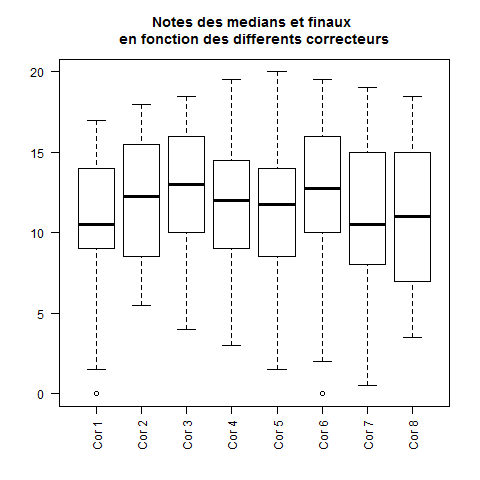
\includegraphics[width=5cm]{correcteurs-notes.png}
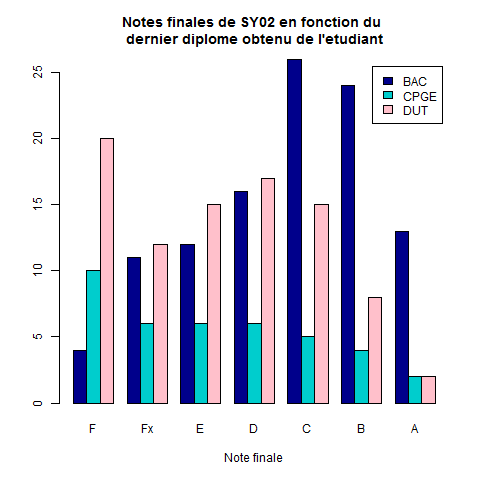
\includegraphics[width=5cm]{diplome-notes.png}
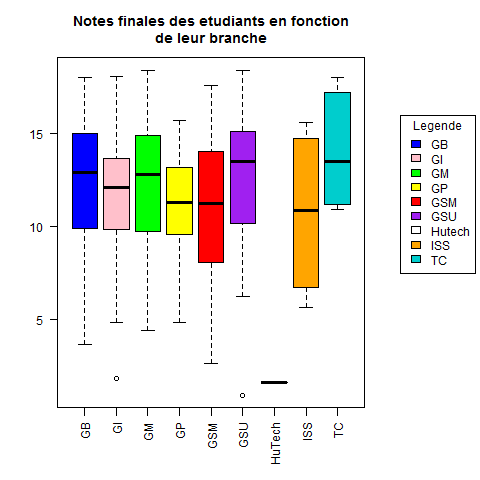
\includegraphics[width=5cm]{branche-notes.png}
\end{center}
\end{figure}
\subsection{Données crabs}
\subsubsection{}
Le jeu de données se compose de 200 observations sur des crabes qui décrivent 7 variables différentes: 2 variables qualitatives et 3 variables quantitatives. Les variables qualitatives décrivent les caractéristiques suivantes: le sexe du crabe (F ou M) et l'espèce du crabe (O ou B). Ci-dessous la représentation des différentes variables qualitatives en fonction des crabes male/female et des crabes d'espèces orange/blue.
\begin{figure}[H]
\begin{center}
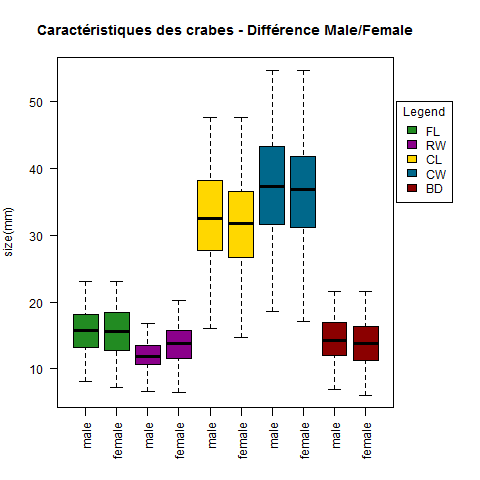
\includegraphics[width=8cm]{caracteristiquesMF.png}
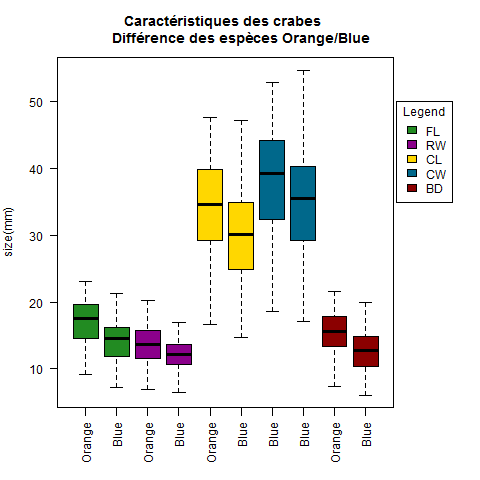
\includegraphics[width=8cm]{caracteristiquesOB.png}
\end{center}
\end{figure}
Ce que l'on peut retenir de ces graphiques c'est qu'il n'y a pas une caractéristique qui détermine si une espèce est un mâle ou une femelle et de même pour les espèces. On peut remarquer que quelques caractéristiques sont plus déterminantes que d'autres: par exemple la taille du lobe frontal (FL) est bien plus élevée pour les crabes de l'espèce orange. Cependant pour chaque caractéristique on remarque que les deux boîtes à moustache se chevauchent donc on ne peut pas se fier à cette première analyse pour identifier le sexe ou l'espèce grâce à une des caractéristiques.
\paragraph{}
Pour aller plus loin dans l'analyse, nous pouvons comparer deux à deux chaque caractéristique grâce à la fonction $plot$ sur la matrice $crabsquant$.
\begin{figure}[H]
\begin{center}
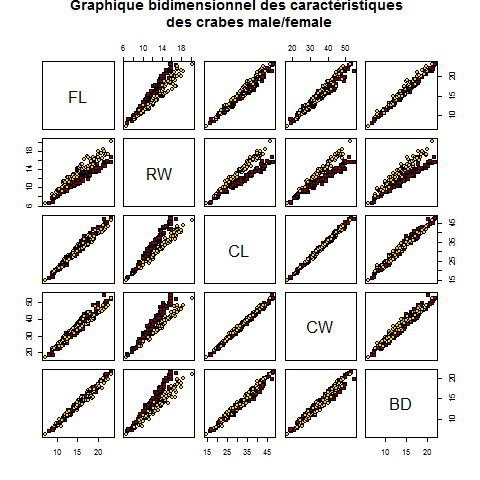
\includegraphics[width=8cm]{sexe-crabs.png}
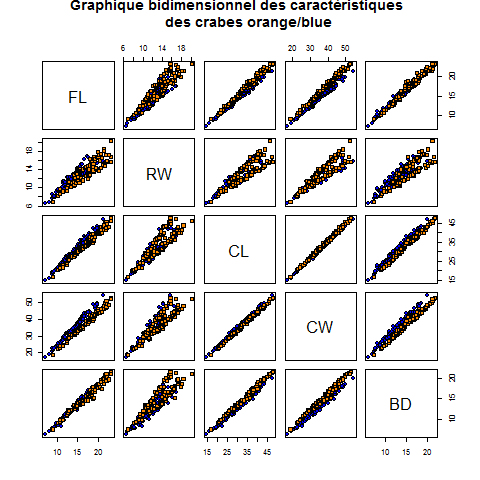
\includegraphics[width=8cm]{spicies-crabs.png}
\end{center}
\end{figure}
On remarque qu'il existe une forte liaison entre toutes les caractéristiques. Même avec ce graphe bidimensionnel, il est difficile de distinguer les mâles des femelles ou les espèces Orange des espèces Blue.
\subsubsection{}

\section{Conclusion}
\end{document}
